\section{Design}
I dette afsnit vil overvejelser, beslutninger og resultater vedrørende softwarearkitektur, subsystemdesign og design af persistens blive beskrevet. 

\subsection{Softwarearkitektur}
\subsubsection{Overvejelser}
Da projektcasen blev fremlagt fra gruppen var der bred enighed om, at lave et system der lægger tæt op ad det oprindelig forslag. I projektcasen fremgik et forslag til en systemtegning, som kan ses på figur \ref{fig:tv2_system}. Et sådan system ville indeholde et REST api, som i dette projekt er uden for scope, og dette brugte gruppen meget tid på at diskutere. Hvis projektet skulle omhandle et REST api, måtte det ikke gå ud over kvaliteten på resten af projektet, og hvis det på et tidspunkt viste sig, at det ikke ville være muligt at implementere api'et, skulle det skrottes og der skulle findes en anden løsning. For at vise krediteringerne til brugerene, blev det overvejet om der skulle laves en wepapplikation og en desktop-klient. Både system- og kanaladministratore, producere, royalty brugere og gæster ville skulle have adgang til denne del af system. For at hente data om kanaler og produktioner, blev det overvejet om der skulle laves en EPG poller, der ville hente data fra TVTid.dk, og derved få alle kanaler og deres tilhørende produktioner. 

\subsubsection{Beslutninger}
På baggrund af gruppens overvejelser blev det valgt af sætte et nyt domæne diagram op over systemet der viser hvordan opsætningen er tiltænkt. I systemet bliver det en REST API der binder hele systemet sammen. REST API vil håndtere input fra Desktop-client gennem subsystemet flask og sende samt hente information fra databasen via subsystemet SQLAlchemy. 

\subsubsection{resultater}
Ud fra beslutningerne kunne dannes et Domændediagram af software arkitekturen som kan ses på figur \ref{fig:domaindiagram-software-diagram}.\\

\begin{figure}[h]
    \centering
    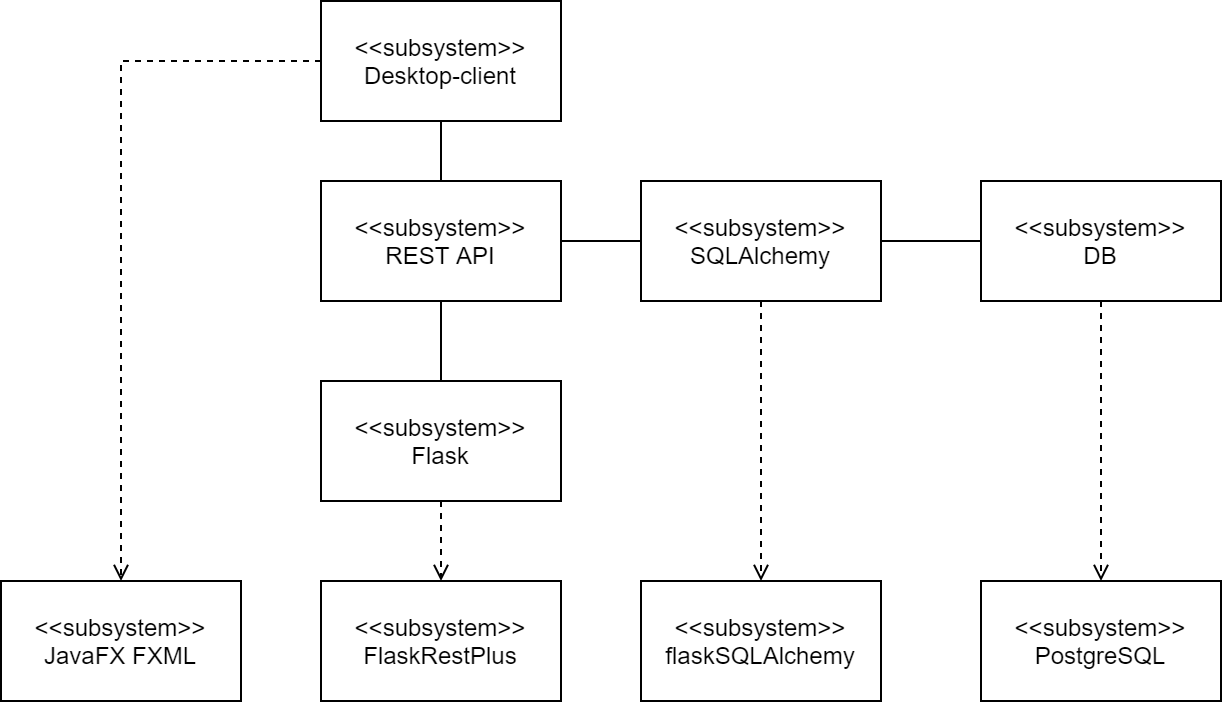
\includegraphics[width=\textwidth]{figures/design/domaindiagram-Software Architecture Diagram.png}
    \caption{Domænediagram Software Arkitektur Diagram}
    \label{fig:domaindiagram-software-diagram}
\end{figure}{}

På diagrammet kan de forskelliges subsystemer relationer ses samt de afhænigheder de har. 

\subsection{Subsystemdesign}
\subsubsection{API}
\subsubsection{Overvejelser}
Processen for design og implementationen var ret klar, da en af vores gruppe medlemmer arbejder med dette. Dog var prioriteringen af rækkefølgen som API'et skulle implementeres i, noget der blev overvejet nøje. 

\subsubsection{Beslutninger}
For at undgå udviklings blockers for de andre systemer der skulle interagere med API'et (desktop klienten, og EPG Polleren) besluttede vi at lave alle endpointsne først, og senere implementere hvilke bruger roller det kræves for de forskellige operationer.

\subsubsection{Resultater}
Vi besluttede at udvide vores designklassediagram for API'et en smule ved at sætte labels på hvilke endpoint, de forskellige metoder for hver klasse hører til. På den måde var det let at se for de andre applikationer at se, hvad de kunne forvente af hvert endpoints.

\subsubsection{Desktop Klient}
\subsubsection{Overvejelser}
Den overvejelse der fyldte mest var beslutningen omkring hvilket designmønstre, vi skulle designe vores applikation med hensyn til.\\
I undervisningen er vi blever undervist i et simplificeret designmønster, der opdeler applikationen i tre lag; præsentation, domæne - og persistens lag. Hvor domæne laget indeholder alt vores forretningslogik. En anden mulighed der minder lidt om denne er MVC (model-view-controller), der også indeler systemet i tre lag, eller MVVM (model-view-viewmodel), hvor viewet ikke kender noget til modellen og vice versa, men i stedet forbindes via viewmodel laget, og hvor det meste UI kan opdateres fra viewmodel laget gennem to-vejs data-bindings.

\subsubsection{Beslutninger}
Vi endte med at benytte MVVM mønstret, da det trods dets overhead at sætte op, vil være et godt valg til vores applikation og gruppe. Vi kunne godt se det smarte i at kunne udvikle på view delen (view controller og FXML) separat fra vores viewmodel og model lag. Samt er det også fedt at man yderligere kan opdele arbejdet med viewmodel og modellen, efter man har designet en "kontrakt" ved at blive enige om de forskellige metoder modellen skal implementere i et interface.

\subsubsection{Resultater}
Ud over de tre lag, lavede vi også en netværksmappe der står for at kommunikere med API'et. Ved at separere denne logik har vi også haft mulighed for at udvikle på desktop klienten sideløbende med API'et. Da vi blot kunne lave en "dummy" klient, der returnerer statiske objekter, i stedet for det faktiske data som den får fra API'et. \\

Ud fra de nye opdagelser i forhold til design kunne analysemodelen opdateres til en design klassemodelsom kan findes i bilag \ref{appendices: desktop-client_domainmodel}.


\subsubsection{EPG-Poller}
\subsubsection{Overvejelser}
\subsubsection{Beslutninger}
\subsubsection{Resultater}


\subsection{Persistens design}
Da persistens skulle designes, var der en stor overvejelse om hver klient skulle have deres egen database, eller om der skulle stræbes efter at få et mere virkelighedstro system (et system der vil afspejle det TV2 lagde op til), der indeholder en centraliseret database. Det blev valgt at stræbe efter det sidstnævnte, og i forbindelse med dette blev der foretaget et valgt at kommunikationen mellem klient og database skulle foregå gennem et REST API så klienterne ikke har direkte adgang til databasen. På denne måde sikres det også at brugere af systemet kun kan foretage de handlinger som deres respektive rolle giver adgang til, da valideringen ligger på server-siden (så brugeren ikke har muglighed får at sniffe brugernavn og kode til databasen og få adgang af andre veje).